\chapter{Benchmarking HYADES} \label{app:benchmark}

\minitoc

In this appendix, a series of benchmarking simulations are presented. HYADES simulations were performed (using the same settings as used for the main simulation campaigns in this thesis) of experimental shots performed at Omega and the NIF, in order to assess the accuracy of the simulations. This benchmarking was not intended to be exhaustive, but to give some indication of whether the settings used in these simulations were sufficient to describe real experimental data.

\section{Direct-drive Omega shots}

The first benchmarking simulations were of 10 calibration shots, performed in a direct-drive configuration on OMEGA. These shots were performed as part of a study of diffusion-dominated mixing \cite{Zylstra2018a}. The 10 shots simulated here used capsules containing different HT vapour mixtures, surrounded by either a pure CH shell or a CH shell with 2\% D. The shells used in these shots were homogeneous, and did not have the multi-layer structure described in \cite{Zylstra2018a}. Each shot was simulated using the same settings as described for the main simulation campaign, including the 0.8 multiplier applied to the input laser energy to estimate the impact of CBET. The simulation results were then compared to the absorbed laser energy, DT and TT yields, along with the bang time and burn width for the three experimental shots where this was recorded.

\begin{figure}[ht]
\centering
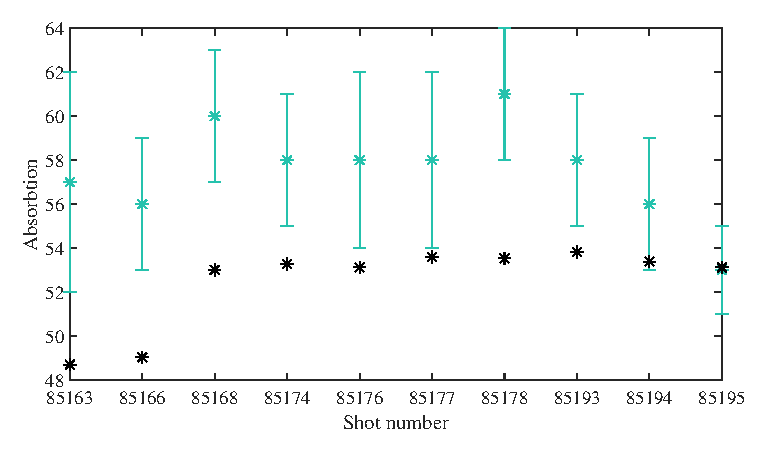
\includegraphics{figures/LowCR/BenchmarkOmegaAbsorbtion.eps}
\caption{Fractional absorption of the laser energy measured in simulation (black) and experiment (teal). The simulated data is obtained by measuring the absorption within the simulation, and multiplying this value by the 0.8 input power multiplier used to account for CBET.}
\label{fig:OmegaAbs}
\end{figure}

\begin{figure}[ht]
\centering
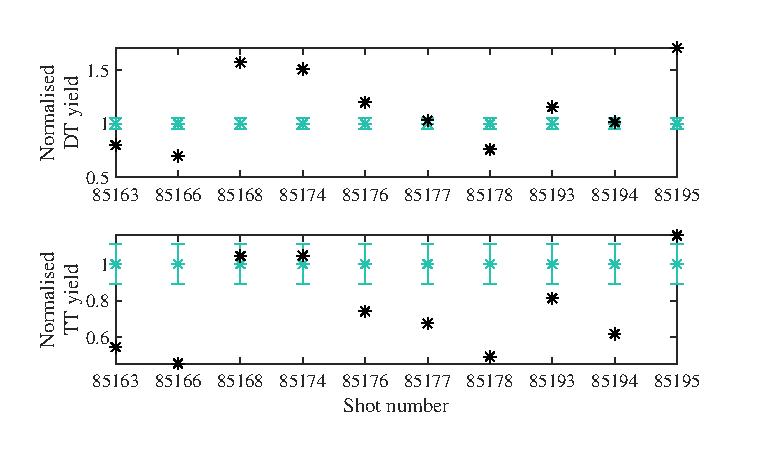
\includegraphics{figures/LowCR/BenchmarkOmegaYield.eps}
\caption{DT and TT yields for the different OMEGA shots, normalised to the experimental data. The black points are the normalised simulated data, while the teal points with a consistent value of 1 are the normalised experimental data, included to show the error bars.}
\label{fig:OmegaYield}
\end{figure}

The simulated and experimental fractional laser absorption for each of the ten shots is displayed in Figure \ref{fig:OmegaAbs}. In almost all cases, the simulated absorption underestimates that seen in the experiment, and lies just outside the error. This could be improved by increasing the value of the CBET multiplier. However, the discrepancy is relatively small (at most 6 \%), and so given the 1D nature of these simulations this level of agreement is likely sufficient (especially as underestimating this value means that the simulations are more pessimistic, rather than exaggerating performance).

Figure \ref{fig:OmegaYield} shows the DT and TT neutron yields, normalised to the experimental performance (for this reason, the experimental data points all have a value of 1; they are included simply to show the error). The normalised DT yield has a mean of 1.14 and varies between approximately 0.7 and 1.7, while the normalised TT yield has a mean of 0.76 and varies between approximately 0.4 and 1.2. While there is some clear variation in these values (which should be expected, given the 1D nature of these simulations), it is clear that generally the simulations are providing a reasonable prediction of the experimental performance. It is notable that the simulated TT yield significantly underestimates the experimental yield, while the DT yield is a slight overestimate. This could possibly be indicative of kinetic effects such as fuel stratification \cite{Bellei2014}; such effects are not included in hydrodynamics codes, and it is known that neglecting them can lead to an underestimation of TT yields \cite{Casey2012}.


\begin{figure}[ht]
\centering
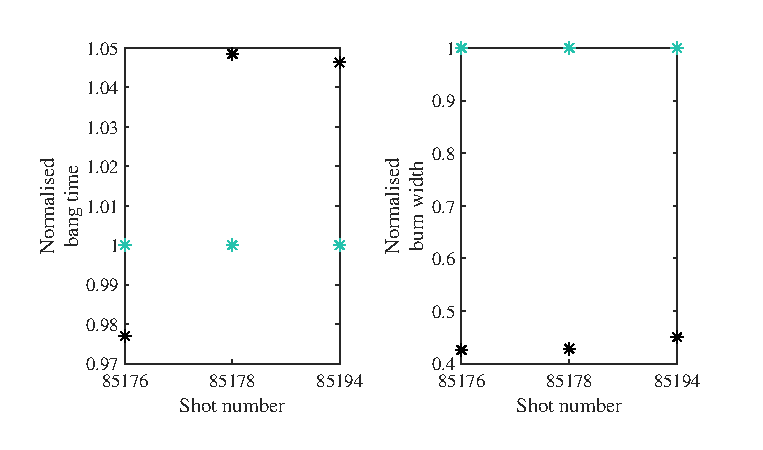
\includegraphics{figures/LowCR/BenchmarkOmegaBT.eps}
\caption{Bang time and burn width for the different OMEGA shots, normalised to the experimental value. The orange/grey points are the normalised simulated data, while the blue/black points with a consistent value of 1 are the normalised experimental data.}
\label{fig:OmegaBT}
\end{figure}


Figure \ref{fig:OmegaBT} displays the bang time and burn width (both normalised to the experimental values for each shot). The normalised simulated bang time varies between 0.97 and 1.05, showing close agreement with the experimental value. The normalised simulated burn width however varies between 0.4 and 0.5, and therefore significantly underestimates the experimental results. It is possible this could be due to a difference in definition of burn width; the FWHM of the neutron production rate was used for the simulated results, but details were not provided on how this was calculated from the experimental data.

Overall, these results suggest that the HYADES simulations, using these settings and a laser absorption multiplier of 0.8, were sufficient to provide a reasonable estimate of experimental performance in these OMEGA shots. The TT yield and burn width were underestimated, but such parameters are not particularly important for the work discussed in this thesis. The simulations were generally able to match the bang time, laser absorption, and DT yield relatively closely; while there was some variation in the DT yield (and the laser absorption was a slight underestimate), this is to be expected given the 1D nature of the code.

\section{Polar direct-drive NIF shot}

Further benchmarking was performed by simulating the NIF shot N190227, based on data provided by Dr Brian Haines \cite{NIFshot}. This was a polar direct-drive shot, and so tested how well such simulations could describe a shot in such a configuration. The capsule was filled with DT vapour at a pressure 6000 torr (64\% D, 36\%T), with a 25~\si[per-mode=symbol]{\micro\meter} CH ablator and an  outer diameter of 3943~\si[per-mode=symbol]{\micro\meter}. The laser ramped linearly from 0 to 400 TW over 1.5ns, remained at this power for 2 ns, and then decreased to 0 TW over 0.5 ns. It produced a DT yield of \num{1.11e16} neutrons (no error was given for this value), a bang time of 4.51 $\pm$ 0.03 ns, and a burn width of 468 $\pm$ 50 ps. The same simulation settings were used as for the main simulation campaigns and OMEGA benchmarking, but a range of different input power multipliers were used (in expectation that the PDD configuration would result in lower laser absorption).


\begin{figure}[ht]
\centering
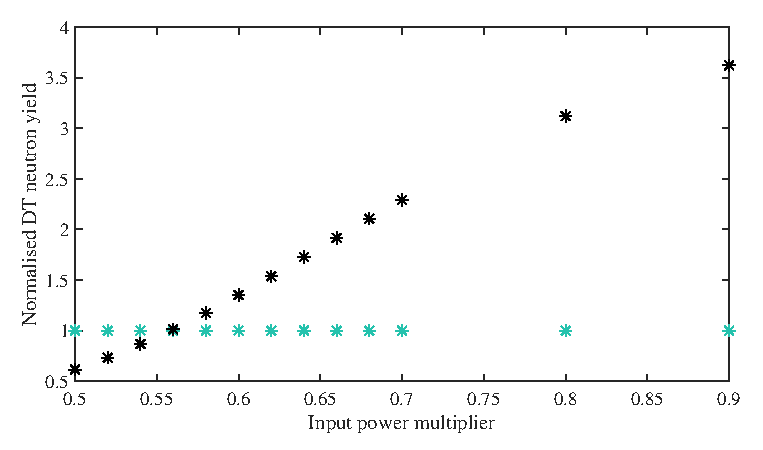
\includegraphics{figures/LowCR/BenchmarkNifYield.eps}
\caption{DT yield for NIF shot N190227 simulated using a range of input power multipliers, normalised to the experimental value of \num{1.11e16}. The black points are the normalised simulated data, while the teal points with a consistent value of 1 are the normalised experimental data.}
\label{fig:NIFYield}
\end{figure}

\begin{figure}[ht]
\centering
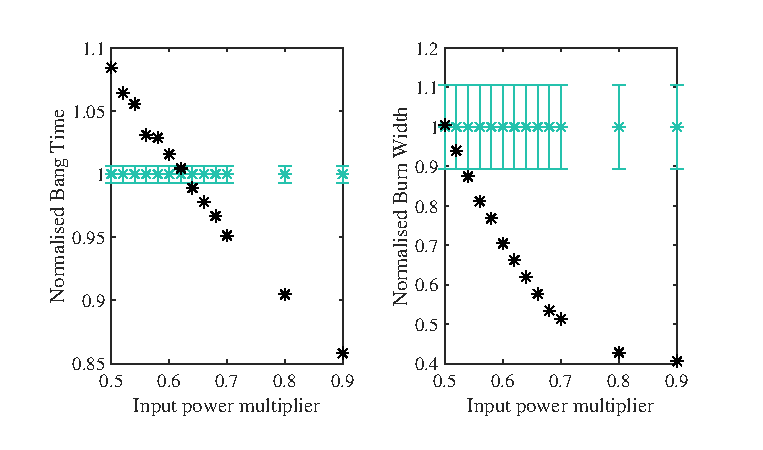
\includegraphics{figures/LowCR/BenchmarkNifBangTime.eps}
\caption{Bang time and burn width for NIF shot N190227 simulated using a range of input power multipliers, normalised to the experimental values of 4.51 $\pm$ 0.03 ns and 468 $\pm$ 50 ps respectively. The black points are the normalised simulated data, while the teal points with a consistent value of 1 are the normalised experimental data.}
\label{fig:NIFBT}
\end{figure}

The simulated and experimental DT yield, normalised in each case to the experimental value, is displayed as a function of the laser power multiplier in Figure \ref{fig:NIFYield}. The best agreement is observed for multipliers between 0.54 and 0.58, while the multiplier of 0.8 (used for the OMEGA symmetric direct-drive benchmarking) results in a DT yield three times higher than measured experimentally. The normalised bang-time and burn-widths can be seen in Figure \ref{fig:NIFBT}. The bang-time shows much better agreement for all input multipliers, but shows the closest agreement (between 1.05 and 0.95) for multipliers ranging between 0.56 to 0.7. The best agreement is observed for a multiplier of 0.62. The burn width is to within the experimental error only for the lowest multipliers used here of 0.5 and 0.52 (although agreement would also likely be observed at slightly lower values as well). For a multiplier of 0.6 the burn width is approximately 0.7 times that of the experimental value, whilst for a multiplier of 0.8 this falls to around 0.4.

There is no single multiplier which perfectly describes all three data sets, but reasonable agreement for all is seen for input multipliers of 0.55 to 0.6. This is significantly lower than the input multiplier of 0.8 which was sufficient to well describe the OMEGA shots. This difference is to be expected based on the PDD configuration; PDD is well-known to suffer from decreased absorption compared to spherically symmetric direct-drive shots, and is particularly susceptible to cross-beam energy transfer. Overall, these simulations of NIF shot N190227 suggest that the simulations presented here can be used to provide a reasonable estimate of polar direct-drive experimental performance, but that a lower laser input multiplier is required to account for the reduced laser absorption. These additional losses mean that when simulating a PDD configuration, either reduced performance should be expected, or the laser input power is required to be around 30 \% higher to achieve the same performance. 

\section{Conclusions}

The results in this section show that spherically-symmetric direct-drive OMEGA experimental shots could be described with reasonable accuracy using HYADES with the settings used in this thesis, including a laser input power modifier of 0.8. However, simulating a polar direct-drive NIF shot required a lower multiplier in the range of 0.55-0.6, with a multiplier of 0.8 significantly overestimating the fusion yield. This is likely due to the reduced laser absorption in polar direct-drive. This suggests that simulations performed in HYADES with these settings and a 0.8 input multiplier can be used to obtain reasonable estimates of performance, but that less agreement is expected if a PDD experimental configuration is used.

The benchmarking here is not exhaustive. A relatively small range of capsules and implosions have been considered, and the polar direct-drive results in particular are based on only a single shot; more simulations of experimental data would be required to make firmer conclusions. However, these initial results are sufficient to indicate that the simulation models and settings used throughout this thesis are reasonable, and can be relied on to provide a reasonable level of accuracy.
